\section{Task 2}\label{sec:task2}

The goal of the second task is to implement a software to quantify global differences between ensembles of a PED and, from them, identify the variance level along the sequence. The input of this task are files containing the features of one PED ensemble generated during Task 1.

\subsection{Ensembles features}
Relationships between different ensambles will be identified considering the structural features of single ensemble using the features file of the task 1.

At the begining, the software extracts the features for each ensamble (multiple conformations):
\begin{itemize}
\item Radius of gyration of each model in the ensemble. It may happen that the number of the values returned are less then the number of the ensamble's conformations, then we check on the array dimension and, if needed, a zero-padding is added.
\item Secondary structure entropy for each position across ensemble conformations exploiting its probabilistic definition between the each model. 
\item Median ASA for each position across ensemble's conformations. We extract the ASA vector for each position and then we compute the median of this vector. 
\item Median RMSD using rotate-translation matrices for each conformation.
\item Median distance of each pair of equivalent positions. We consider the columns of conformation distance matrices and we return their median values.
\item Standard deviation of the distances for each positions across all the ensamble's conformations.
\end{itemize}


\subsection{Global metric}
The global metric evaluates the distance between ensembles pairs. It takes into account the different nature of the features evaluated.
This metric return the sum of partial distances of different features:
\begin{itemize}
\item The absolute value of the difference between the mean radius of gyration for the two ensembles.
\item The Chebyshev distance between the entropies of the two ensembles. It finds the distance as the greatest of their differences along any coordinate dimension.
\item The euclidean distance between the median ASA of the two ensembles.
\item The euclidean distance between the median RMSD of the two ensembles.
\item The complementary of the correlation between the median distance of the two ensembles.
\end{itemize}


Using the global metric just described, the software displays the distances between two ensembles through:
\begin{itemize}
\item Heatmap: it calculates the matrix of the distances between the features of the ensambles and then builds and displays the heatmap. The distance between ensembles is highlighted with different colors based on the similarity scale reported on the right. 
\item Dendrogram: using a linkage matrix and the presented global metric, the dendrogram built combining the most similar ensembles with respect to the calculated features (with a 'complete' approach) is plot.
\end{itemize}

\begin{figure}[H]
	\begin{minipage}[b]{0.93\textwidth}
		\centering
		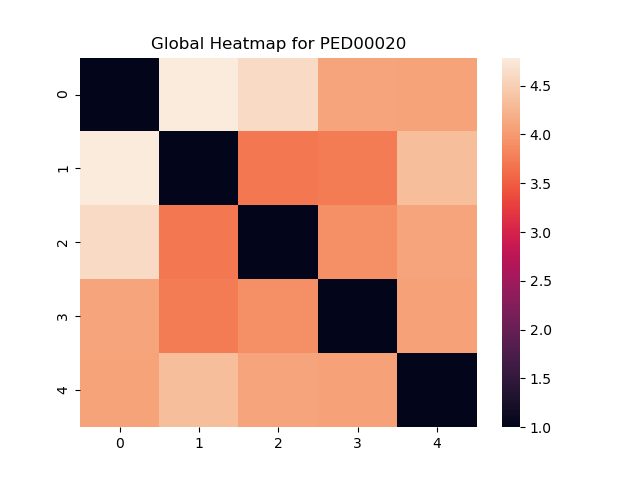
\includegraphics[width=\textwidth]{PED00020_heatmap.png}
		\caption{Heatmap of all the model.}
		\label{heatmap}
	\end{minipage}
\end{figure}
\begin{figure}
	\begin{minipage}[b]{0.93\textwidth}
		\centering
		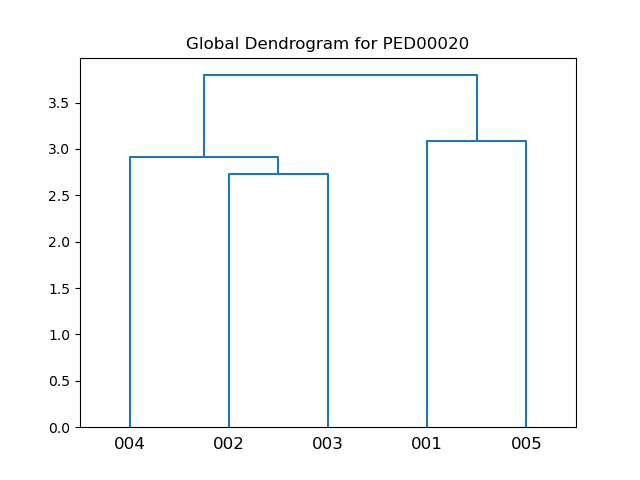
\includegraphics[width=\textwidth]{PED00020_dendrogram.png}
		\caption{Dendrogram of all the model.}
		\label{dendrogram}
	\end{minipage}
\end{figure}

In figures \ref{heatmap} and \ref{dendrogram}, it is possible to visualize respectively the distance and similarity between the five ensemblesù. It can be observed that ensembles 1 and 2 are the most similar while ensemble 4 is the most distant.


\subsection{Local metric}
The local metric evaluates the variability of all the features for each position in the ensemble.
This metric computes the mean of the total values for each residues with respect all the ensamble features: %Presentazione della metrica non mi convince tanto
\begin{itemize}
\item Total Entropy is the standard deviation of the conformations entropy for each position.
\item Total median ASA is the standard deviation of the conformations accessible surface area for each position.
\item Total median RMSD is the standard deviation of the conformations median RMSD for each position.
\item Total standard deviation of distance is the trimmed mean of the conformations median RMSD for each position. 
The use of a trimmed mean helps eliminate the influence of outliers or data points on the tails on the traditional mean.
\end{itemize}

\begin{figure}[H]
	\begin{minipage}[b]{0.97\textwidth}
		\centering
		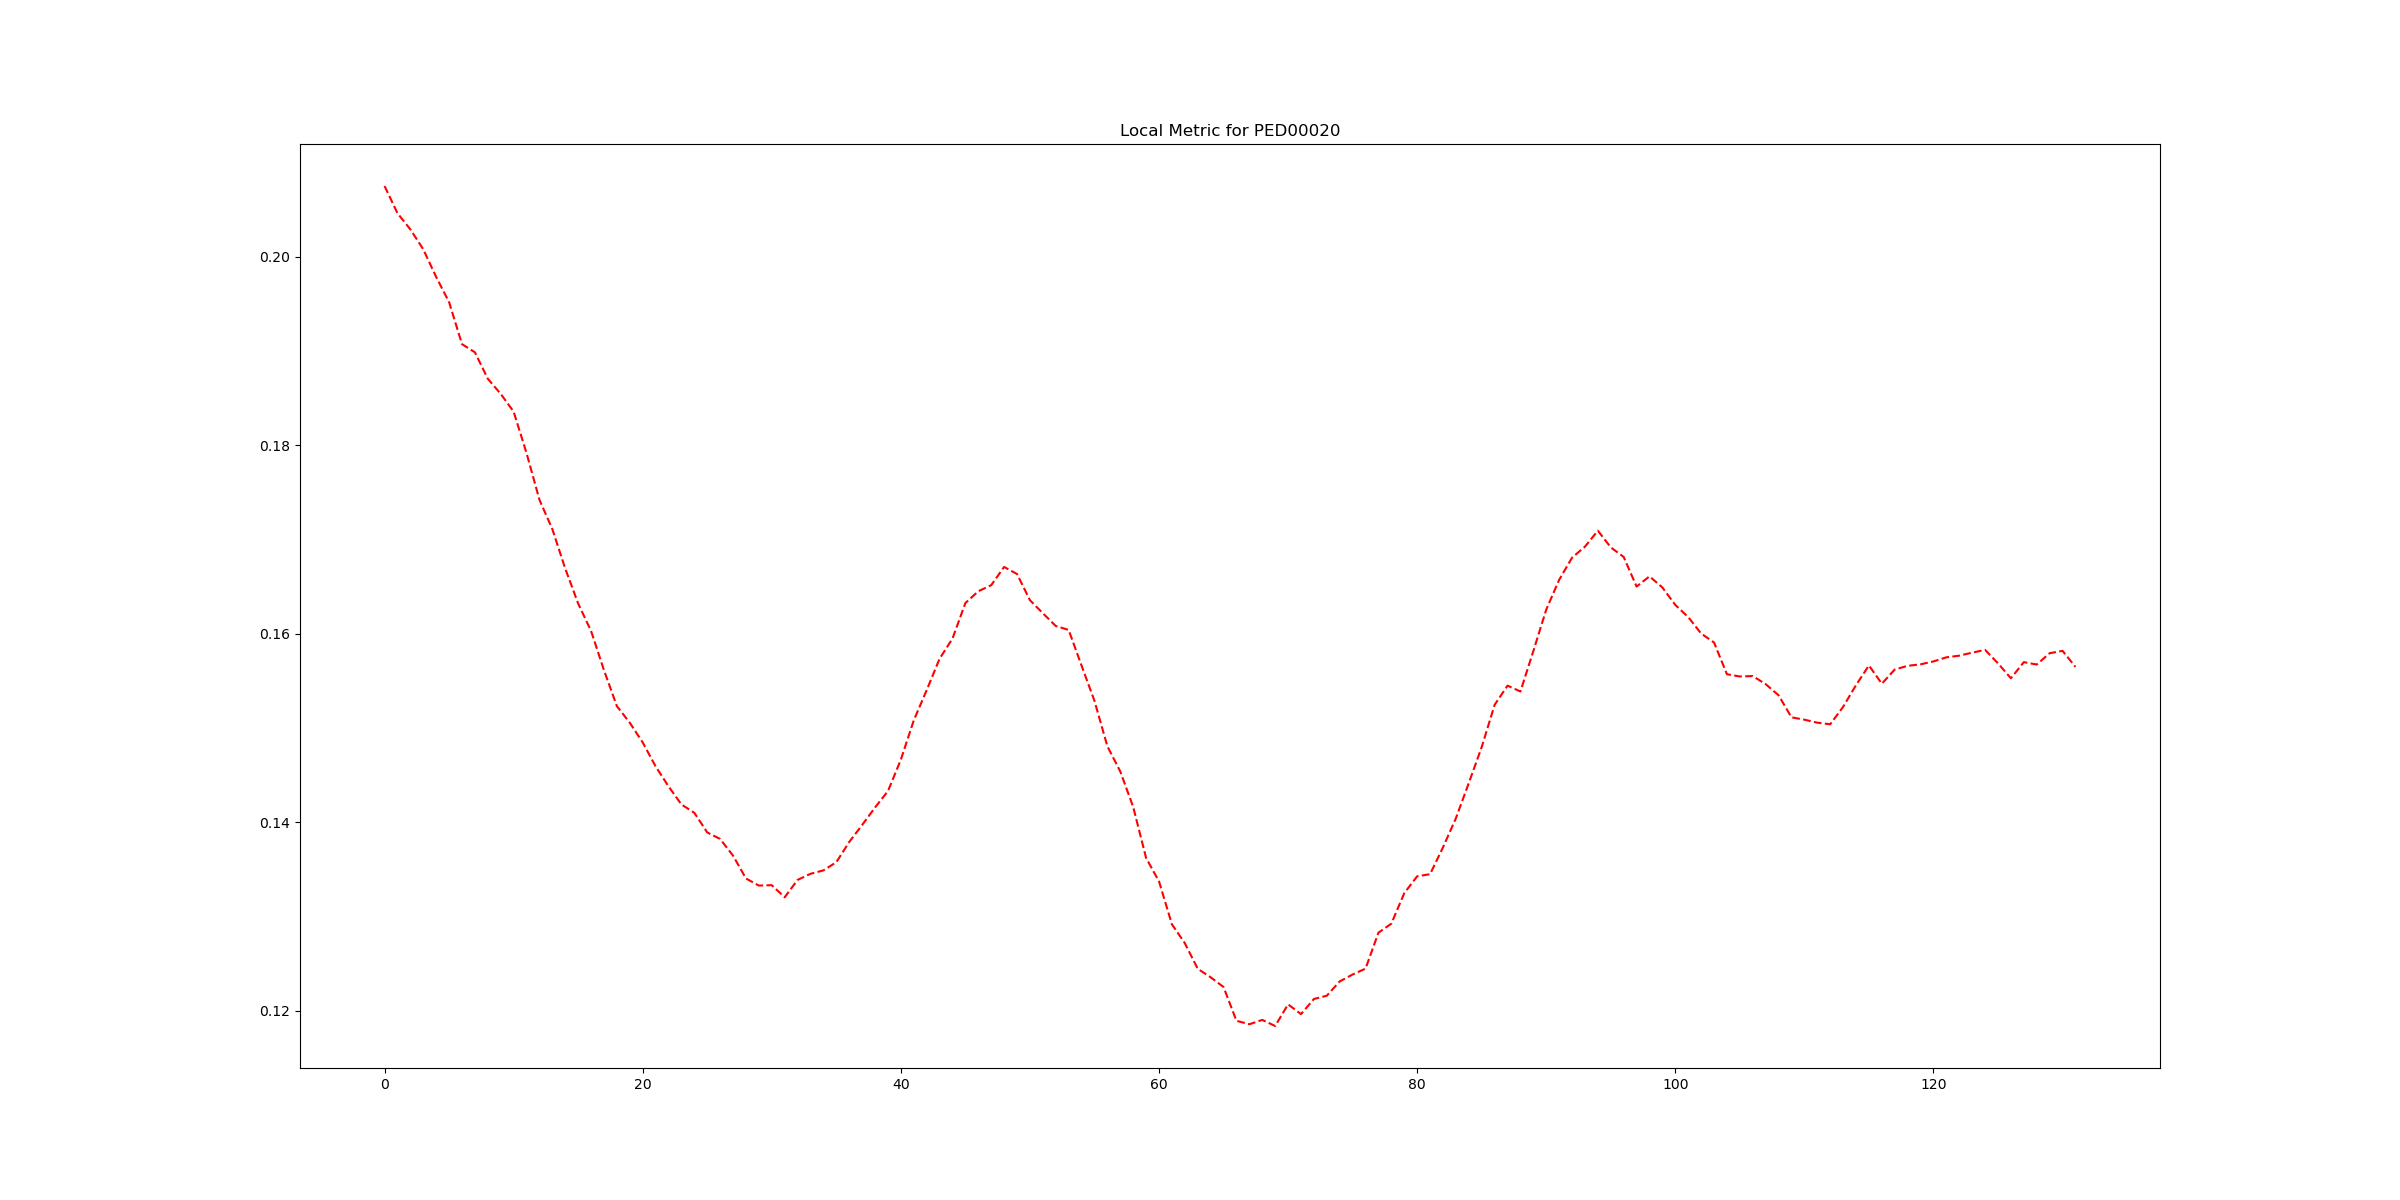
\includegraphics[width=\textwidth]{PED00020_local.png}
		\caption{Plot of local features.}
		\label{plot}
	\end{minipage}	
\end{figure}
In \ref{plot} it is possible to visualize the ensembles features variation for each residue using the local metric. 

Looking at the graph above and taking into consideration the information extracted from the various comparisons in this project, we can conclude that the structure of the measles virus nucleoprotein is quite disordered in the initial part where the variability is greater. Furthermore, there is a continuous change in the variability of local distances within the structure. There are minimum points where even more defined structures can be identified through pymol images (e.g. alpha-helix).%Riportare maggiore correlazione con Pymol?